\section{Measurement of Thermal Energy}

\begin{multicols}{2}


\section*{Specific Heat Capacity}


\subsection[Specific Heat Capacity of Liquids]{Specific Heat Capacity of \hfill \\ Liquids}

\begin{center}
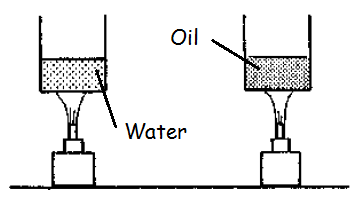
\includegraphics[width=0.4\textwidth]{./img/source/shc-liquids.png}
\end{center}

\begin{description*}
%\item[Subtopic:]{}
\item[Materials:]{\nameref{sec:heatsources}, 2 containers, water, oil}
%\item[Setup:]{}
\item[Procedure:]{Heat equal masses of different liquids (e.g. water and oil) in two identical containers for the same length of time.}
\item[Hazards:]{Take great care not to overheat the oil, as it can catch fire. Do not touch if you have heated it for a long time.}
\item[Questions:]{What difference in temperature can you feel with your finger?}
%\item[Observations:]{}
\item[Theory:]{The temperature of the oil is higher because it needs less energy to raise the temperature of one gram of oil by 1$^\circ$C than that of water. Thus, using the same amount of heat and mass, the temperature of the oil must be higher.}
%\item[Applications:]{}
%\item[Notes:]{}
\end{description*}

\subsection{Mass and Thermal Energy}

\begin{center}
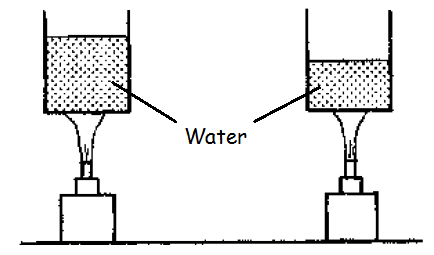
\includegraphics[width=0.4\textwidth]{./img/source/thermal-energy.png}
\end{center}

\begin{description*}
%\item[Subtopic:]{}
\item[Materials:]{\nameref{sec:heatsources}, 2 containers, water}
%\item[Setup:]{}
\item[Procedure:]{Heat different quantities of water in two identical containers (e.g. tin cans) for the same length of time. Dip your finger into the two containers of water.}
%\item[Hazards:]{}
\item[Questions:]{What difference in temperature can you feel?}
%\item[Observations:]{}
\item[Theory:]{The temperature of the smaller quantity of water is higher, because it received more thermal energy per gram of its mass than the larger quantity. So for the same heat input the temperature rise of the smaller quantity of water will be greater.}
%\item[Applications:]{}
%\item[Notes:]{}
\end{description*}

\subsection{The Calorimeter}

\begin{center}
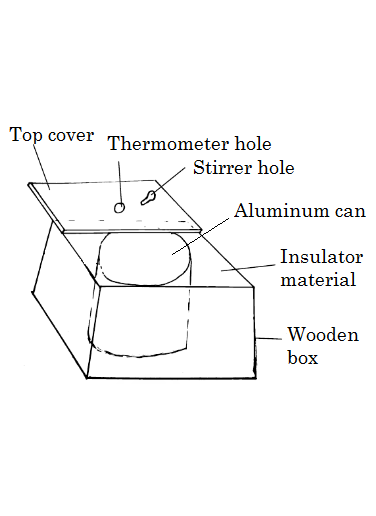
\includegraphics[width=0.49\textwidth]{./img/calorimeter.png}
\end{center}

\begin{description*}
%\item[Subtopic:]{}
\item[Materials:]{Wooden box (10 cm $\times$ 10 cm $\times$ 12 cm), ceiling board/piece of wood, aluminum can, aluminum wire, pieces of blanket/sweater, thermometer}
\item[Setup:]{Prepare a wooden box with a cover from wood or ceiling material. Use aluminum wire to make a stirrer with a rubber holder.}
\item[Procedure:]{Place the piece of blanket in the box as an insulator, then the aluminum can with stirrer. Place the top cover on the box, followed by stirrer holder and thermometer in the middle hole.}
%\item[Hazards:]{}
%\item[Questions:]{}
%\item[Observations:]{}
\item[Theory:]{To measure specific heat capacity, a liquid of known mass and temperature is added to the container (e.g. water) and a solid or liquid of known mass and temperature (and unknown specific heat capacity) is added to the liquid.}
\item[Applications:]{The specific heat capacity, $c$ of the object can be found by using the relationship $(mc\Delta T)_{object} = (mc\Delta T)_{al} + (mc\Delta T)_{w}$, where $c_{al}$ and $c_{w}$ are known for aluminum and water and all masses and temperatures are measured.}
\item[Notes:]{The can and stirrer must be of the same material.}
\end{description*}

\vfill
\columnbreak

\subsection[Determining Specific Heat Capacity of a Liquid]{Determining Specific Heat \hfill \\ Capacity of a Liquid}

%\begin{center}
%\includegraphics[width=0.4\textwidth]{./img/source/.png}
%\end{center}

\begin{description*}
%\item[Subtopic:]{}
\item[Materials:]{Thermometer, water, any liquid, \nameref{sec:meascyl}, small pot, glass jar, \nameref{sec:heatsources}}
%\item[Setup:]{}
\item[Procedure:]{Measure a known volume of the liquid into a glass container. Heat the water in the pot over a stove until it is significantly warmer than the other liquid. Measure the volume of the water in the measuring cylinder. Before mixing the liquids, measure each temperature and record it. Now pour the hot water into the other liquid and wait for the temperature of the mixture to equalize. When the temperature levels off, measure and record it.}
%\item[Hazards:]{}
\item[Questions:]{Determine the specific heat capacity of the liquid.}
%\item[Observations:]{}
\item[Theory:]{Since the liquid and water are being mixed, the same amount of heat energy $H$ used to raise the liquid’s temperature is lost by the water to cool it down. Thus $H_w = H_l$, or $(mc\Delta T)_{w} = (mc\Delta T)_{l}$. The masses of the substances are known from their densities or measured, and the changes in temperature are measured with the thermometer. The specific heat capacity of water is 4200 J/kg K, so the specific heat capacity of the liquid can be found.}
%\item[Applications:]{}
%\item[Notes:]{}
\end{description*}

\subsection{Application of Specific Heat Capacity}

\begin{center}
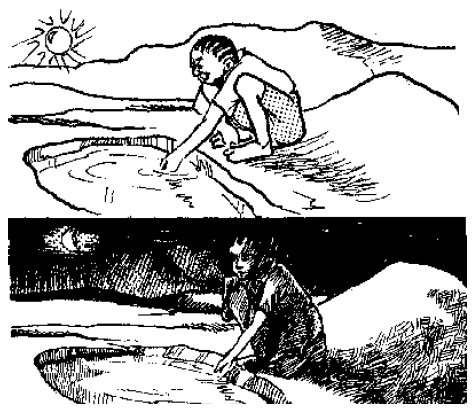
\includegraphics[width=0.4\textwidth]{./img/source/shc-app.png}
\end{center}

\begin{description*}
%\item[Subtopic:]{}
%\item[Materials:]{}
%\item[Setup:]{}
\item[Procedure:]{Use your hand to find out how fast a water puddle and a heap of sand warm up during the day and cool during the night.}
%\item[Hazards:]{}
%\item[Questions:]{}
\item[Observations:]{The sand heats up faster during the day and cools down faster at night.}
\item[Theory:]{Sand has a lower specific heat capacity than water ($c_{water} = 4200$ J/kg K, $c_{sand} = 800$ J/kg K), and so less heat energy is required to change its temperature.}
%\item[Applications:]{}
%\item[Notes:]{}
\end{description*}

%==================================================================================================%

\section*{Change of State}

There are three states of matter, \emph{solid}, \emph{liquid} and \emph{gas}. Matter can be converted from one state to another:

\begin{center}
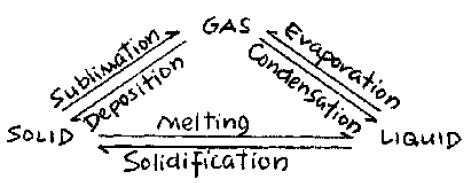
\includegraphics[width=0.49\textwidth]{./img/source/change-of-state.png}
\end{center}

%For more, see the the From I topic \nameref{sec:states-matter}.

\subsection{Condensation}

\begin{center}
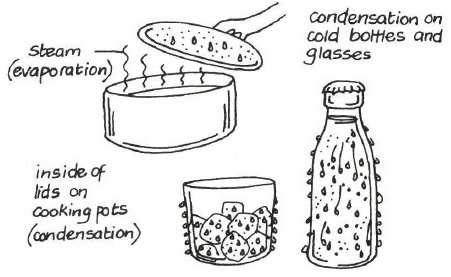
\includegraphics[width=0.49\textwidth]{./img/vso/condensation.jpg}
\end{center}

Condensation occurs when a gas (e.g. water vapour) cools down and becomes a liquid.

\subsection{Bottle Condensation}

\begin{center}
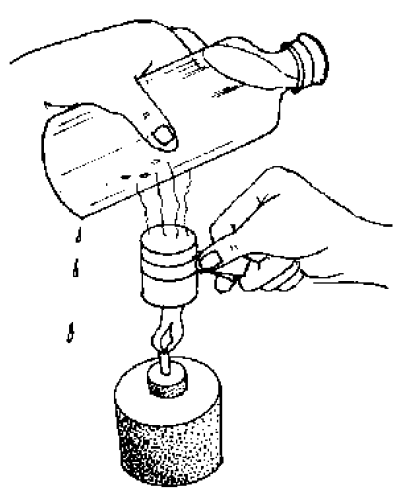
\includegraphics[width=0.25\textwidth]{./img/source/change-state.png}
\end{center}

\begin{description*}
%\item[Subtopic:]{}
\item[Materials:]{Tin can, glass bottle, water, \nameref{sec:heatsources}}
%\item[Setup:]{}
\item[Procedure:]{Pour a small amount of water into a tin can and heat it until it boils. Fill a bottle with cool water and hold it above the tin can.}
%\item[Hazards:]{}
%\item[Questions:]{}
\item[Observations:]{Water drops form on the outside of the cool bottle when it is touched by the steam of the boiling water.}
\item[Theory:]{Water particles escape from the boiling water as vapour and condense on the lower surface of the bottle to form water droplets. Hence water is made up of small particles.}
%\item[Applications:]{}
%\item[Notes:]{}
\end{description*}

\columnbreak

%==================================================================================================%

\section*{Melting Point}


\subsection{Determining Melting Point}

\begin{center}
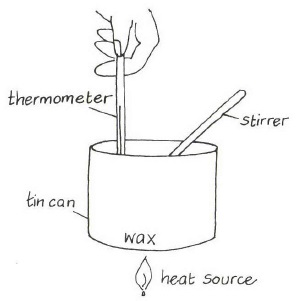
\includegraphics[width=0.4\textwidth]{./img/vso/melting-point.jpg}
\end{center}

\begin{description*}
%\item[Subtopic:]{}
\item[Materials:]{Tin can, thermometer, stirrer, \nameref{sec:heatsources}, candle wax}
%\item[Setup:]{}
\item[Procedure:]{Gently melt the wax, stirring continuously to make sure the thermometer does not rest on the bottom of the tin. Record the temperature at which all of the wax has melted.}
%\item[Hazards:]{}
%\item[Questions:]{}
\item[Observations:]{You should notice that the temperature remains constant until all the wax has melted, then begins to rise.}
\item[Theory:]{The point at which the temperature changes is the melting point.}
\item[Applications:]{Collect several temperatures over time and make a temperature-time graph for wax.}
%\item[Notes:]{}
\end{description*}

%\subsection{Pressure and Melting Point}
%
%\begin{center}
%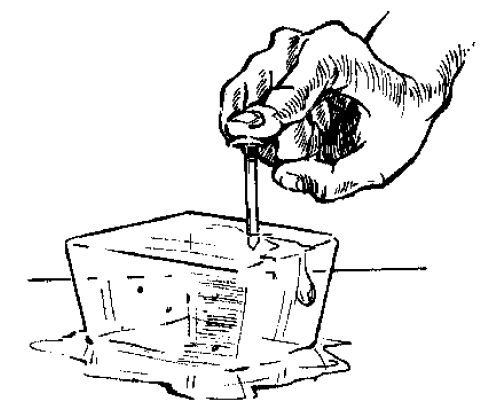
\includegraphics[width=0.4\textwidth]{./img/source/pressure-melting-point.png}
%\end{center}
%
%\begin{description*}
%%\item[Subtopic:]{}
%\item[Materials:]{Nail, block of ice}
%%\item[Setup:]{}
%\item[Procedure:]{Steadily press a nail into a block of ice without heating it.}
%%\item[Hazards:]{}
%%\item[Questions:]{}
%%\item[Observations:]{}
%\item[Theory:]{The nail penetrates into the ice because the pressure causes the ice at the tip of the nail to melt. This is because water has less volume than the same mass of ice. But when you release the pressure on the nail, the water freezes again and ``glues'' the nail into the block of ice.}
%%\item[Applications:]{}
%%\item[Notes:]{}
%\end{description*}

%==================================================================================================%

\section*{Boiling Point}


\subsection{Impurities and Boiling Point}

%\begin{center}
%\includegraphics[width=0.4\textwidth]{./img/source/.png}
%\end{center}

\begin{description*}
%\item[Subtopic:]{}
\item[Materials:]{Tin can, salt, \nameref{sec:heatsources}, thermometer}
%\item[Setup:]{}
\item[Procedure:]{Add water and a small amount of salt to a container and heat over a stove. Measure the temperature at which the water boils.}
%\item[Hazards:]{}
%\item[Questions:]{}
\item[Observations:]{The water boils at a temperature slightly higher than 100$^\circ$C when salt is added.}
\item[Theory:]{Impurities such as salt increase the boiling point of water.}
\item[Applications:]{Adding salt causes water to take a longer time to begin boiling, but when it does boil it is at a higher temperature and thus can cook food faster.}
%\item[Notes:]{}
\end{description*}

\columnbreak

\subsection[Boiling Water at Room Temperature]{Boiling Water at Room \hfill \\ Temperature}

\begin{center}
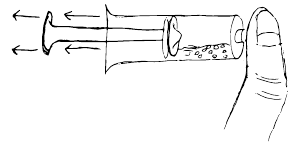
\includegraphics[width=0.4\textwidth]{./img/boiling-room-temp.png}
\end{center}

\begin{description*}
%\item[Subtopic:]{}
\item[Materials:]{Syringe (10 mL or 20 mL), water}
%\item[Setup:]{}
\item[Procedure:]{Fill the syringe with a small amount of water. Place your thumb over the opening and pull the plunger out as far as you can.}
%\item[Hazards:]{}
%\item[Questions:]{}
\item[Observations:]{When the plunger is pulled back the water begins to bubble, meaning that it is boiling.}
\item[Theory:]{The pressure inside the syringe decreases, and the boiling point of water is decreasing with the pressure. When the boiling point is reduced to room temperature, the water begins to boil.}
%\item[Applications:]{}
\item[Notes:]{The activity will not work if you use too much water.}
\end{description*}

\subsection{Pressure Cooker}

\begin{center}
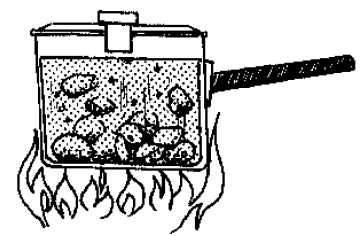
\includegraphics[width=0.4\textwidth]{./img/source/pressure-cooker.png}
\end{center}

\begin{description*}
%\item[Subtopic:]{}
%\item[Materials:]{}
%\item[Setup:]{}
%\item[Procedure:]{}
%\item[Questions:]{}
%\item[Observations:]{}
\item[Theory:]{Under the high pressure in such a pot the water boils at a higher temperature of about 120$^\circ$C. At this temperature food like beans need only about one hour (instead of 3 in a normal pot) to cook and become soft. Therefore the pressure cooker uses less fuel to cook.}
\item[Applications:]{At high altitudes air pressure decreases, and thus water boils at a lower temperature. So food would need a very long time to be cooked (e.g. at the top of Mount Kilimanjaro). To cook food faster we need to use a pressure cooker to increase the temperature inside.}
\item[Hazards:]{Do not try to make a homemade pressure cooker as it can easily explode.}
%\item[Notes:]{}
\end{description*}

\columnbreak

%==================================================================================================%

\section*{Evaporation}


\subsection{Evaporation and Cooling}

\begin{center}
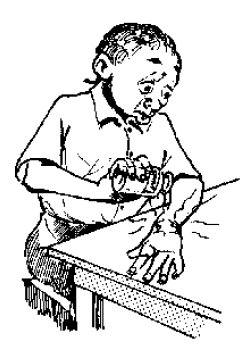
\includegraphics[width=0.3\textwidth]{./img/source/evap-cooling.png}
\end{center}

\begin{description*}
%\item[Subtopic:]{}
\item[Materials:]{Petrol/spirit (e.g. Konyagi)}
%\item[Setup:]{}
\item[Procedure:]{Pour some petrol or spirit on the back of your hand.}
%\item[Hazards:]{}
%\item[Questions:]{}
%\item[Observations:]{}
\item[Theory:]{The back of the hand feels cold, because evaporation of the spirit needs energy which it absorbs from the skin.}
\item[Applications:]{When you go swimming and come out of the water, you feel cold because evaporation of water from your body absorbs heat from your skin. This is also why the body produces sweat in order to cool down.}
%\item[Notes:]{}
\end{description*}

\subsection{Cooling Water}

\begin{center}
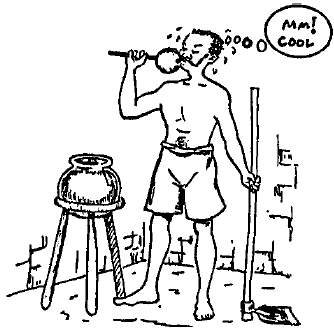
\includegraphics[width=0.4\textwidth]{./img/source/cooling-water.png}
\end{center}

\begin{description*}
%\item[Subtopic:]{}
%\item[Materials:]{}
%\item[Setup:]{}
%\item[Procedure:]{}
%\item[Hazards:]{}
%\item[Questions:]{}
%\item[Observations:]{}
\item[Applications:]{In many houses water is kept in fired clay pots (\emph{chungu}). They have very tiny pores through which minute amounts of water ooze out.}
\item[Theory:]{Some water passes through the tiny pores and evaporates. The energy needed for the evaporation is taken from the pot and water and hence the water cools down.}
%\item[Notes:]{}
\end{description*}

\subsection{Latent Heat of Vaporisation}

%\begin{center}
%\includegraphics[width=0.4\textwidth]{./img/source/.png}
%\end{center}

\begin{description*}
%\item[Subtopic:]{}
\item[Materials:]{\nameref{sec:heatsources}, water, small pot, thermometer}
%\item[Setup:]{}
\item[Procedure:]{Fill the pot half-way with water and heat with a thermometer inside. Record the temperature every 10 seconds after the water begins to boil.}
%\item[Hazards:]{}
\item[Questions:]{Plot a graph of temperature (vertical axis) against time (horizontal axis).}
\item[Observations:]{The temperature increases steadily as the water is heated, then upon boiling remains constant while the water vapourizes. The graph will show a steadily increasing temperature until it reaches the boiling point on the vertical axis (about 100$^\circ$C. At this point, the temperature will level off as time continues to increase.}
\item[Theory:]{When a substance is heated, its temperature increases as it gains heat as per its heat capacity. However, when it changes state from solid to liquid or liquid to gas, its temperature remains constant as it is absorbing latent heat.}
%\item[Applications:]{}
%\item[Notes:]{}
\end{description*}

\subsection{Distillation}

\begin{center}
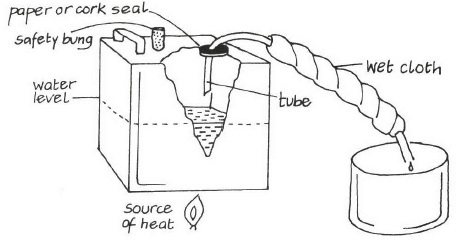
\includegraphics[width=0.49\textwidth]{./img/vso/distillation.jpg}
\end{center}

\begin{description*}
%\item[Subtopic:]{}
\item[Materials:]{Metal can, cork/rubber stopper, plastic tubing, wet cloth, container, \nameref{sec:heatsources}}
%\item[Setup:]{}
\item[Procedure:]{Fill a container half way with water. Cut a hole in the top and fix a rubber stopper with a plastic tube through the center. Wrap a wet cloth around the tube and feed it into a can. Add a safety bung using rubber or cork to prevent against very high pressures within the container and place the container over the heat source.}
\item[Hazards:]{Make sure the safety bung is not too tight and that the container always has water inside.}
%\item[Questions:]{}
%\item[Observations:]{}
\item[Theory:]{Heating the can produces steam which is then cooled by the wet cloth. Steam condenses to produce water.}
\item[Applications:]{This method can be used to purify water.}
%\item[Notes:]{}
\end{description*}

%==================================================================================================%


\end{multicols}

\pagebreak